\documentclass[preprint,12pt]{elsarticle}

\usepackage{amsmath,amssymb,bm}
\usepackage{booktabs,array}
\usepackage{graphicx}
\usepackage{xurl}
\usepackage{hyperref}
\usepackage{pdflscape}
\hypersetup{hidelinks}
\setlength{\emergencystretch}{3em}
\graphicspath{{figures/}{../../05_results/}}

\begin{document}

\begin{center}
{\Large Supplementary Material}\par\medskip
{\large Finite-time perturbation selection in evolving HCP crystal plasticity:\\
path-dependent direction, wavelength and mechanism}
\end{center}

\section{Complete fixed-candidate norm--selector screen}

Figure~\ref{fig:s_full_matrix} reports the complete terminal 11-by-7 screen
that was previously summarized by representative columns.  Each cell gives
the winning log gain and abbreviated branch label among the three registered
onset-$x$, onset-$y$ and terminal-$y$ candidates.  This figure is a
fixed-candidate sensitivity screen; it is not the re-optimized result in
Section~\ref{sec:s_reoptimized}.

\clearpage
\begin{landscape}
\begin{figure}[p]
\centering
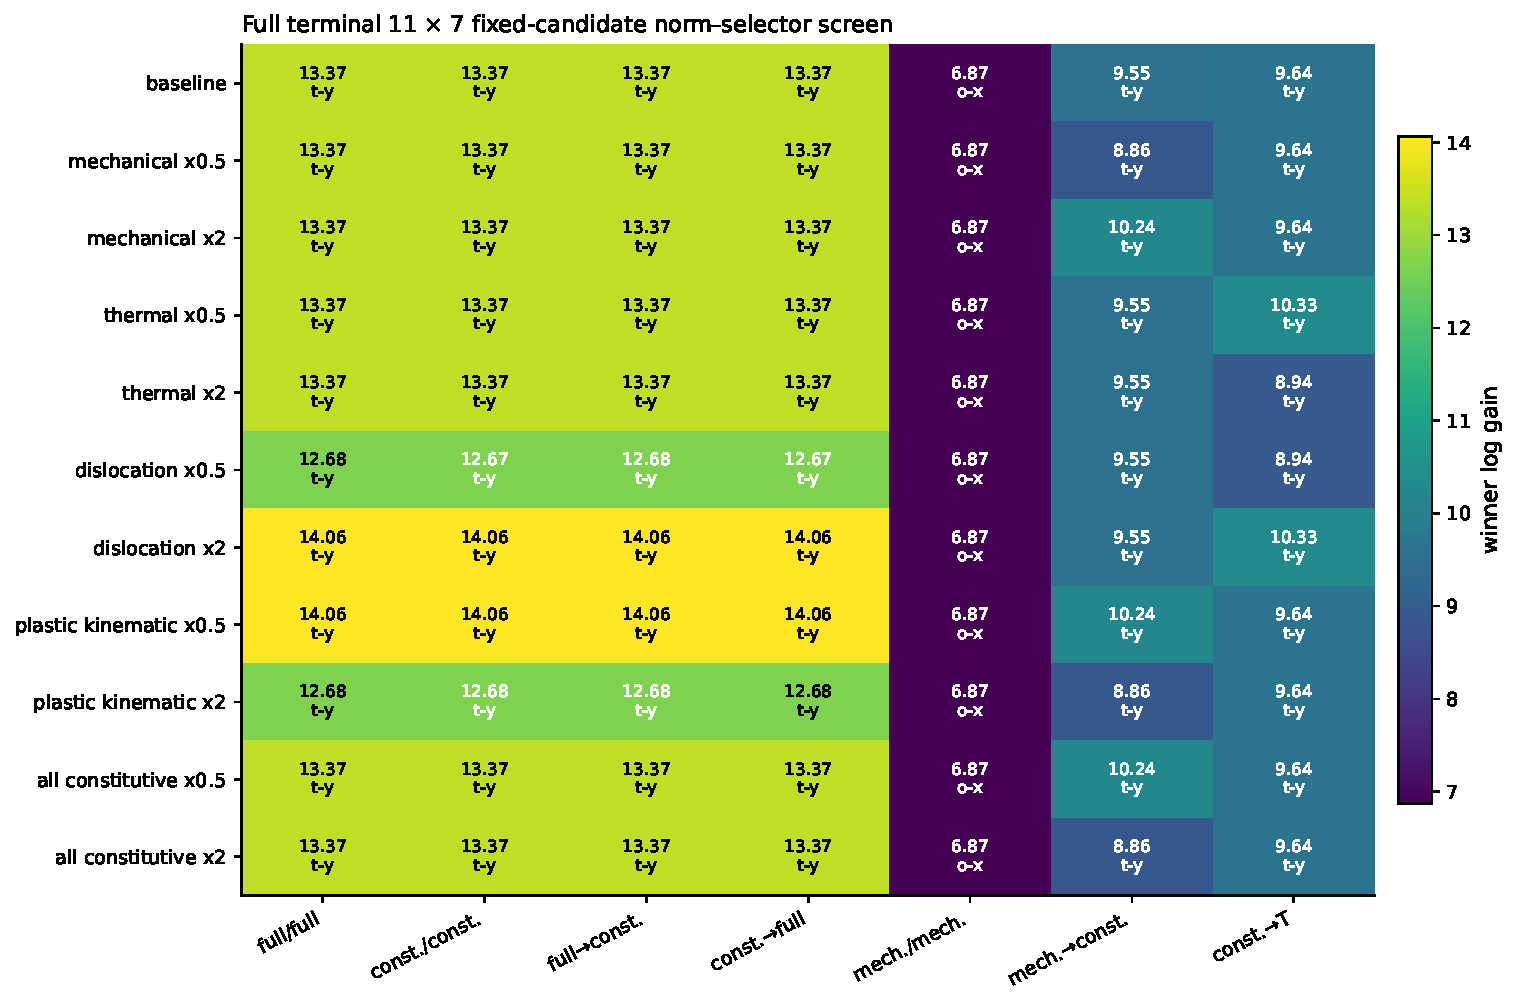
\includegraphics[width=0.92\linewidth]{figS01_full_norm_selector_matrix.pdf}
\caption{Complete terminal fixed-candidate norm--selector matrix. The rows are
the baseline norm and ten factor-two coordinate-scale perturbations; the
columns are all seven declared input--output maps. Cell annotations report
log gain and the winning registered branch.}
\label{fig:s_full_matrix}
\end{figure}
\end{landscape}
\clearpage

\section{Re-optimized direction--wavenumber and matched freezing}
\label{sec:s_reoptimized}

Direction and wavenumber are re-optimized for all seven selectors under the
baseline and four pre-registered adverse norms.  The singular-value audit
applies the formal 5\% relative-gap threshold, and the piecewise-frozen audit
uses exactly the same metric and endpoint selectors as the time-ordered map.
Machine-readable coordinates, gains, complete singular values/vectors,
baseline generators, convergence rows and all optimizer evaluations are
supplied in \path{05_results/ijp_revision_evidence_v3/} and
\path{05_results/ijp_revision_evidence_v3_arrays.npz}.  The synthesized figure
is included in the main paper rather than duplicated here.

\section{Loading transfer, local sensitivity and titanium landmarks}

The V3 table directory supplies the three added loading cases, the
branch-local $\pm20\%$ sensitivity records and logarithmic derivatives, and
the bounded external check against synchronized Grade-II CP-Ti
stress/temperature landmarks.  The latter is a timing-and-scale check, not a
batch-calibrated validation.  The figure synthesized from those tables is
included in the main paper.

\section{Reproducibility contracts}

The complete V3 receipt is
\path{05_results/ijp_revision_evidence_v3.json}.  The exact literature
landmarks and extraction record are under
\path{04_reproducibility/literature_digitization/guo2019_prl/}.  Parameter
source keys S4 and S5 identify the exact paper, frozen kernel version, public
repository commit, configuration paths, SHA-256 checksums and access date.

\end{document}
